\documentclass{minimal}
\usepackage{bm}
\usepackage{epsfig,color}
\usepackage[papersize={576.00bp,432.00bp},text={576.00bp,432.00bp}]{geometry}
\begin{document}
\centering
% Title: glps_renderer figure
% Creator: GL2PS 1.3.8, (C) 1999-2012 C. Geuzaine
% For: Octave
% CreationDate: Wed Jul 29 11:41:12 2015
\setlength{\unitlength}{1pt}
\begin{picture}(0,0)
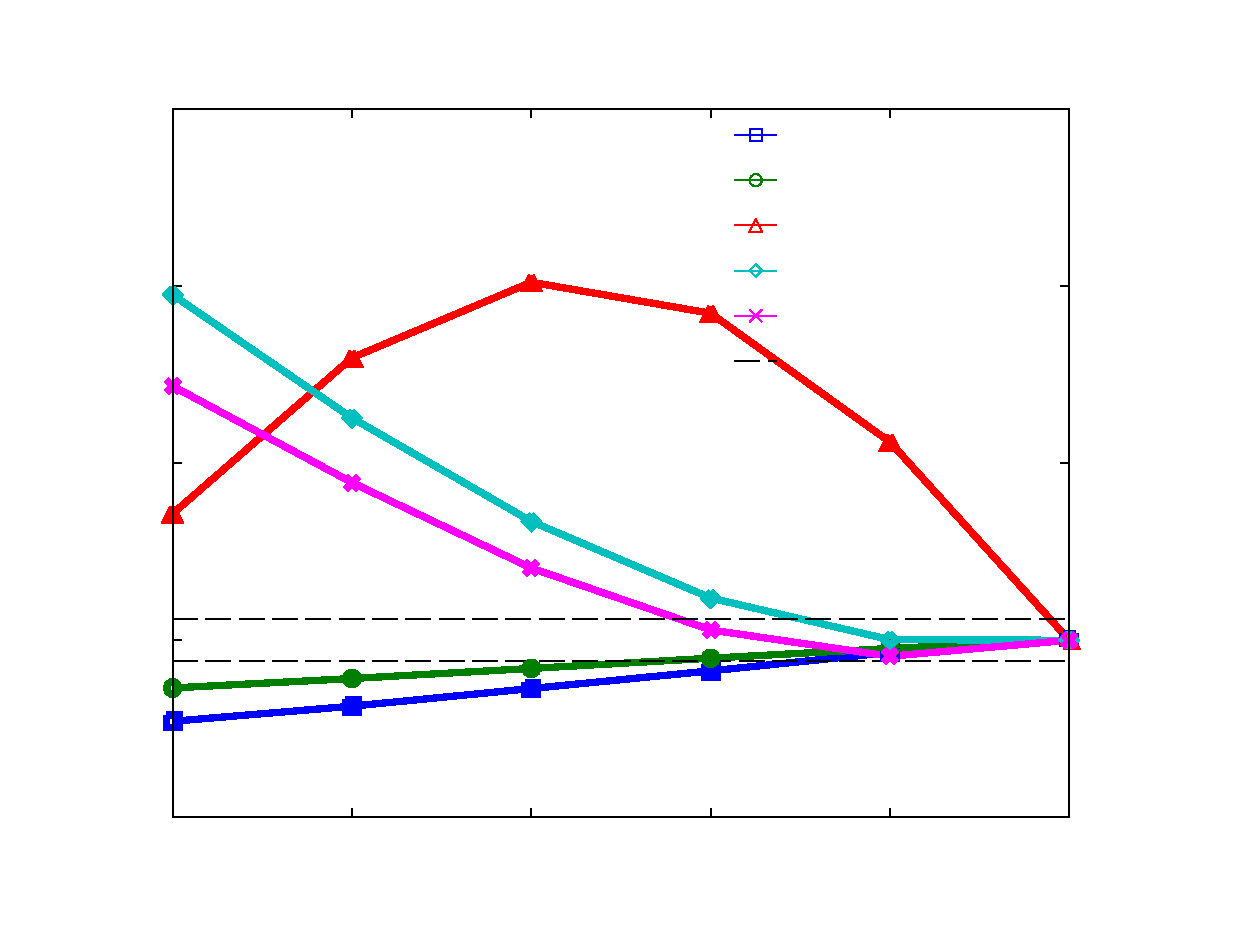
\includegraphics{fig_c2p-inc}
\end{picture}%
\begin{picture}(576,432)(0,0)
\fontsize{16}{0}
\selectfont\put(74.88,42.5188){\makebox(0,0)[t]{\textcolor[rgb]{0,0,0}{{1}}}}
\fontsize{16}{0}
\selectfont\put(160.96,42.5188){\makebox(0,0)[t]{\textcolor[rgb]{0,0,0}{{2}}}}
\fontsize{16}{0}
\selectfont\put(247.04,42.5188){\makebox(0,0)[t]{\textcolor[rgb]{0,0,0}{{3}}}}
\fontsize{16}{0}
\selectfont\put(333.12,42.5188){\makebox(0,0)[t]{\textcolor[rgb]{0,0,0}{{4}}}}
\fontsize{16}{0}
\selectfont\put(419.2,42.5188){\makebox(0,0)[t]{\textcolor[rgb]{0,0,0}{{5}}}}
\fontsize{16}{0}
\selectfont\put(505.28,42.5188){\makebox(0,0)[t]{\textcolor[rgb]{0,0,0}{{6}}}}
\fontsize{16}{0}
\selectfont\put(69.8753,47.52){\makebox(0,0)[r]{\textcolor[rgb]{0,0,0}{{-5}}}}
\fontsize{16}{0}
\selectfont\put(69.8753,132.54){\makebox(0,0)[r]{\textcolor[rgb]{0,0,0}{{0}}}}
\fontsize{16}{0}
\selectfont\put(69.8753,217.56){\makebox(0,0)[r]{\textcolor[rgb]{0,0,0}{{5}}}}
\fontsize{16}{0}
\selectfont\put(69.8753,302.58){\makebox(0,0)[r]{\textcolor[rgb]{0,0,0}{{10}}}}
\fontsize{16}{0}
\selectfont\put(69.8753,387.6){\makebox(0,0)[r]{\textcolor[rgb]{0,0,0}{{15}}}}
\fontsize{16}{0}
\selectfont\put(290.08,29.5188){\makebox(0,0)[t]{\textcolor[rgb]{0,0,0}{{m (bulk cluster size)}}}}
\fontsize{16}{0}
\selectfont\put(53.8753,217.56){\rotatebox{90}{\makebox(0,0)[b]{\textcolor[rgb]{0,0,0}{{$\Delta E_{meth}^m - \Delta E_{meth}^6$ [kcal/mol]}}}}}
\fontsize{16}{0}
\selectfont\put(367.463,374.997){\makebox(0,0)[l]{\textcolor[rgb]{0,0,0}{{nwchem}}}}
\fontsize{16}{0}
\selectfont\put(367.463,353.328){\makebox(0,0)[l]{\textcolor[rgb]{0,0,0}{{abinit}}}}
\fontsize{16}{0}
\selectfont\put(367.463,331.659){\makebox(0,0)[l]{\textcolor[rgb]{0,0,0}{{lammps(RuNNer)}}}}
\fontsize{16}{0}
\selectfont\put(367.463,309.991){\makebox(0,0)[l]{\textcolor[rgb]{0,0,0}{{FHaims}}}}
\fontsize{16}{0}
\selectfont\put(367.463,288.322){\makebox(0,0)[l]{\textcolor[rgb]{0,0,0}{{abinit-neutral}}}}
\fontsize{16}{0}
\selectfont\put(367.463,266.653){\makebox(0,0)[l]{\textcolor[rgb]{0,0,0}{{kT}}}}
\end{picture}
\end{document}
